\documentclass[12pt]{article}

\title{On numerical gravitation}
\author{S. Halayka\footnote{sjhalayka@gmail.com}}
\date{\today\;\currenttime}

\usepackage{datetime}
\usepackage{listings}
\usepackage{cite}
\usepackage{xcolor}
\usepackage{graphicx}
\usepackage{setspace}
\usepackage{amsmath}
\usepackage{url}
\usepackage[margin=0.8in]{geometry}
\usepackage{listings}


\usepackage{xcolor}
\lstset { %
    language=C++,
    backgroundcolor=\color{black!5}, % set backgroundcolor
    basicstyle=\footnotesize,% basic font setting
    showstringspaces=false,
}


%\doublespace

%\usepackage[]{lineno}
%\linenumbers


\begin{document}



 
\maketitle

\begin{abstract}
Abstract.
\end{abstract}




\section{Introduction}

First see \cite{halayka} for a short tutorial for C++ programmers on isotropic Newtonian gravitation.
In \cite{halayka} we build an isotropic gravitational field through the use of pseudorandomly generated field lines.
In \cite{halayka} we use a sphere as the receiver.

In this paper, we find a match between the numerical gravitation and the gravitational time dilation from general relativity \cite{hooft, susskind, misner}.
Here, we use an axis-aligned bounding box (AABB) as the receiver.

In this paper we use Planck units, where $c = G = \hbar = k = 1$, which simplifies the equations.
Note that a length of 1 means 1 Planck length, not 1 metre.


\section{Method}

Where $r_{e}$ is the emitter's Schwarzschild radius, $r_{r}$ is the receiver AABB radius (e.g. half of the AABB side length), $\beta$ is the get intersecting line density function, and $1\mathrm{e}12$ and $0.01$ are arbitrary constants:
\begin{equation}
r_{e} = \sqrt{\frac{1\mathrm{e}12 \log(2)}{\pi}}
\end{equation}
\begin{equation}
r_{r} = r_{e} \times 0.01
\end{equation}
\begin{equation}
A_{e} = 4 \pi r_{e}^2
\end{equation}
\begin{equation}
n_{e} = \frac{A_{e}}{4 \log(2)} = 1\mathrm{e}12
\end{equation}
\begin{equation}
M_{e} = \frac{r_{e}}{2}
\end{equation}

Where $R$ is the distance from the emitter's centre:
\begin{equation}
\alpha = \frac{\beta(R + \epsilon) - \beta(R)}{\epsilon}.
\end{equation}
The gradient strength is:
\begin{equation}
g = \frac{-\alpha}{r_{r}^2} \approx \frac{n_e}{2 R^3}.
\end{equation}
From this we can get the Newtonian acceleration $a_N$:
\begin{equation}
a_N =\frac{g R \log 2}{8 M_{e}} =  \sqrt{\frac{n_e \log 2}{4 \pi R^4}} = \frac{M_{e}}{R^2}.
\end{equation}
We can also get a general relativistic acceleration $a_S$, where $r_e < R$:
\begin{equation}
t = \sqrt{1 - \frac{r_e}{R}},
\end{equation}
\begin{equation}
a_S = \frac{1}{t} \frac{2 M_e}{\pi R^2}.
\end{equation}

\begin{lstlisting}
real_type intersect_AABB(
	const vector_3 min_location, 
	const vector_3 max_location, 
	const vector_3 ray_origin, 
	const vector_3 ray_dir, 
	real_type& tmin, 
	real_type& tmax)
{
	tmin = (min_location.x - ray_origin.x) / ray_dir.x;
	tmax = (max_location.x - ray_origin.x) / ray_dir.x;

	if (tmin > tmax) swap(tmin, tmax);

	real_type tymin = (min_location.y - ray_origin.y) / ray_dir.y;
	real_type tymax = (max_location.y - ray_origin.y) / ray_dir.y;

	if (tymin > tymax) swap(tymin, tymax);
	if ((tmin > tymax) || (tymin > tmax)) return 0;
	if (tymin > tmin) tmin = tymin;
	if (tymax < tmax) tmax = tymax;

	real_type tzmin = (min_location.z - ray_origin.z) / ray_dir.z;
	real_type tzmax = (max_location.z - ray_origin.z) / ray_dir.z;

	if (tzmin > tzmax) swap(tzmin, tzmax);
	if ((tmin > tzmax) || (tzmin > tmax)) return 0;
	if (tzmin > tmin) tmin = tzmin;
	if (tzmax < tmax) tmax = tzmax;
	if (tmin < 0 || tmax < 0) return 0;

	vector_3 ray_hit_start = ray_origin;
	ray_hit_start.x += ray_dir.x * tmin;
	ray_hit_start.y += ray_dir.y * tmin;
	ray_hit_start.z += ray_dir.z * tmin;

	vector_3 ray_hit_end = ray_origin;
	ray_hit_end.x += ray_dir.x * tmax;
	ray_hit_end.y += ray_dir.y * tmax;
	ray_hit_end.z += ray_dir.z * tmax;

	real_type l = (ray_hit_end - ray_hit_start).length();

	return l;
}

vector_3 random_cosine_weighted_hemisphere(const vector_3& normal)
{
	// Generate two random numbers
	real_type u1 = dis(generator);
	real_type u2 = dis(generator);

	// Malley's method (cosine-weighted hemisphere sampling)
	// Sample uniformly on a disk, then project up to hemisphere
	real_type r = sqrt(u1);
	real_type theta = 2.0 * pi * u2;

	// Point on unit disk
	real_type x = r * cos(theta);
	real_type y = r * sin(theta);
	real_type z = sqrt(1.0 - u1); // Height above disk (gives cos weighting)

	// Create orthonormal basis around normal
	vector_3 n = normal;
	n.normalize();

	// Choose an arbitrary vector not parallel to normal
	vector_3 arbitrary;
	if (fabs(n.x) > 0.9)
		arbitrary = vector_3(0, 1, 0);
	else
		arbitrary = vector_3(1, 0, 0);

	// Create tangent and bitangent
	vector_3 tangent = n.cross(arbitrary);
	tangent.normalize();

	vector_3 bitangent = n.cross(tangent);
	bitangent.normalize();

	// Transform from local coordinates to world coordinates
	vector_3 result;
	result.x = tangent.x * x + bitangent.x * y + n.x * z;
	result.y = tangent.y * x + bitangent.y * y + n.y * z;
	result.z = tangent.z * x + bitangent.z * y + n.z * z;

	return result.normalize();
}

std::optional<real_type> intersect(
	const vector_3 location,
	const vector_3 normal,
	const real_type receiver_distance,
	const real_type receiver_radius)
{
	const vector_3 circle_origin(receiver_distance, 0, 0);

	if (normal.dot(circle_origin) <= 0)
		return std::nullopt;

	vector_3 min_location(
		-receiver_radius + receiver_distance, 
		-receiver_radius, 
		-receiver_radius);

	vector_3 max_location(
		receiver_radius + receiver_distance, 
		receiver_radius, 
		receiver_radius);

	real_type tmin = 0, tmax = 0;

	real_type AABB_hit = intersect_AABB(
		min_location, 
		max_location, 
		location, 
		normal, 
		tmin, 
		tmax);

	if (AABB_hit > 0)
		return AABB_hit;

	return std::nullopt;
}

// Beta function, for Newtonian gravitation
real_type get_intersecting_line_density(
	const long long unsigned int n,
	const real_type emitter_radius,
	const real_type receiver_distance,
	const real_type receiver_radius)
{
	real_type count = 0;

	generator.seed(static_cast<unsigned>(0));

	for (long long unsigned int i = 0; i < n; i++)
	{
		if (i % 100000000 == 0)
			cout << float(i) / float(n) << endl;

		const vector_3 p = random_unit_vector();

		vector_3 normal = p;
		vector_3 location = normal;

		location.x *= emitter_radius;
		location.y *= emitter_radius;
		location.z *= emitter_radius;

		std::optional<real_type> i_hit = intersect(
			location, 
			normal, 
			receiver_distance, 
			receiver_radius);

		if (i_hit)
			count += *i_hit / (2.0 * receiver_radius);
	}

	return count;
}

// Beta function, for Schwarzschild gravitation
real_type get_intersecting_line_density(
	const long long unsigned int n,
	const real_type emitter_radius,
	const real_type receiver_distance,
	const real_type receiver_radius)
{
	real_type count = 0;

	generator.seed(static_cast<unsigned>(0));

	for (long long unsigned int i = 0; i < n; i++)
	{
		if (i % 100000000 == 0)
			cout << float(i) / float(n) << endl;

		// Random hemisphere outward
		vector_3 location = random_unit_vector();

		location.x *= emitter_radius;
		location.y *= emitter_radius;
		location.z *= emitter_radius;

		vector_3 surface_normal = location;
		surface_normal.normalize();

		vector_3 normal = random_cosine_weighted_hemisphere(surface_normal);

		std::optional<real_type> i_hit = intersect(location, normal, receiver_distance, receiver_radius);

		if (i_hit)
			count += *i_hit / (2.0 * receiver_radius);
	}

	return count;
}

\end{lstlisting}















\begin{thebibliography}{9}


\bibitem{halayka} Halayka. Newtonian gravitation from scratch, for C++ programmers. (2024)
\bibitem{hooft} `t Hooft. Dimensional reduction in quantum gravity. (1993)
\bibitem{susskind} Susskind. The World as a Hologram. (1994)
\bibitem{misner} Misner et al. Gravitation. (1970)

\end{thebibliography}


\pagebreak





\begin{figure} 
\centering
\label{fig1}
  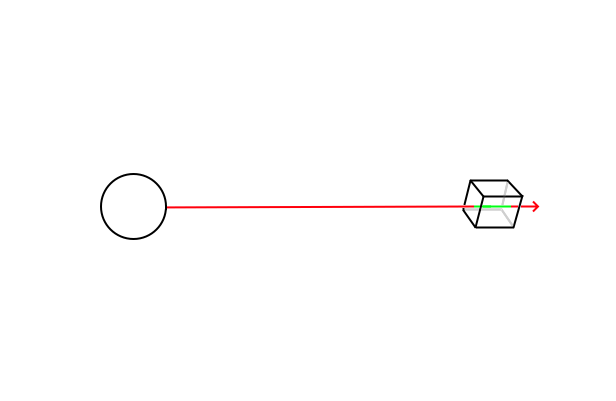
\includegraphics[width =5 in]{AABB.png}
  \caption{
This figure shows an axis-aligned bounding box and an isotropic emitter, looking from slightly above.
An example field line (red) and intersecting line segment (green) are given.
The bounding box is filled with these green intersecting line segments.
It is the gradient of the density of these line segments that forms the gravitational acceleration.
}
\end{figure}`






\end{document}









